\chapter{Background}
\label{chap:background}

Before the individual nowcasting tasks can be defined, two questions have to be
made explicit: what kind of object a time series is, and what assumptions are
introduced when it is transformed into supervised learning data. The background
therefore starts from time-indexed observations, with emphasis on ordering,
sampling, windowing, and the risk of temporal leakage. It then reviews the
machine-learning model families used later in the thesis at the level of their
modeling mechanisms rather than as task-specific experimental choices. On this
basis, a separate section defines the nowcasting problem and the validation
principles needed to assess temporal generalization. The final part returns to
the satellite-link setting, where the technical modeling
problem becomes an operational decision about whether a backup link should be
activated. Detailed model instantiations are left to
\cref{chap:task-formulations}, while training, selection, and evaluation
procedures are left to the experimental setup chapter.

\section{Time Series as Data}
\label{sec:background-time-series}

\subsection{Time Index and Information Order}

A time series is not merely a table with a timestamp column. It is a realization
of a temporal process observed at ordered time instants
\cite{brockwell2016introduction,shumway2017time}. In the setting considered in
this thesis, each observation consists of a timestamp \(t_i\) and a scalar signal
value \(S_i\):
\[
  \{(t_i,S_i)\}_{i=1}^{N},
  \qquad
  t_1 < t_2 < \cdots < t_N .
\]
Equivalently, the measured signal can be interpreted as samples from an
underlying process \(S(t)\), observed only at the finite set of times
\(\{t_i\}_{i=1}^{N}\). The temporal index is therefore part of the data
definition. Two sequences containing the same numerical values but arranged in a
different order can describe different physical evolutions.

Let \(\mathcal{F}_i\) denote the information available at time \(t_i\).
Formally, it is the sigma-algebra generated by \(S_1,\ldots,S_i\): the smallest
sigma-algebra with respect to which these random variables are measurable.
A causal nowcasting model must base its decision at \(t_i\) only
on \(\mathcal{F}_i\). This notation is useful because it separates the offline
construction of labels from the online information set. Future observations may
be used after the fact to define a supervised target, namely the outcome the
model is trained to predict, but they are not part of the information available
when the operational decision is made.

This makes time-series data different from ordinary exchangeable tabular data.
In a tabular classification problem, the rows are often treated as independent
or at least exchangeable after conditioning on their features. In a time series,
row \(i+1\) is not an arbitrary new case: it is the continuation of the same
temporal evolution observed at row \(i\). Models, preprocessing steps, and
validation protocols must respect this direction of time.

\subsection{Temporal Dependence and Non-Stationarity}

Consecutive samples in a time series are statistically dependent. In a satellite-link
signal, the value at \(t_i\) is informative about nearby future values because
atmospheric and equipment states evolve continuously rather than being redrawn
independently at each timestamp. This temporal dependence is the basic reason
why forecasting methods use past observations as input features
\cite{hyndman2021forecasting}.

For a regularly sampled univariate series, second-order temporal dependence is
often summarized through the autocovariance and autocorrelation functions
\cite{shumway2017time}. If the process is weakly stationary, with constant mean
\(\mu\) and variance, the lag-\(k\) autocovariance is
\[
  \gamma(k)
  =
  \operatorname{Cov}(S_i,S_{i-k})
  =
  \mathbb{E}\left[(S_i-\mu)(S_{i-k}-\mu)\right],
\]
and the autocorrelation is
\[
  \rho(k) = \frac{\gamma(k)}{\gamma(0)} .
\]
Positive autocorrelation at small lags means that recent values carry
predictive information about the next samples. For fade nowcasting, this local
dependence is central: an above-threshold sample is operationally more important
when it occurs inside a persistent fade trajectory than when it is an isolated
fluctuation.

Stationarity is a useful reference concept, but real measurement series often
violate it. A strictly stationary process has joint distributions that are
invariant under time shifts, while weak stationarity requires constant first and
second moments and autocovariances that depend only on lag. Satellite-link data
can depart from these assumptions because weather regimes, seasonal effects,
receiver conditions, maintenance interventions, and acquisition quality can
change over long periods. A model trained on one part of the acquisition history
may therefore face a different distribution later in time.

Fade-related signals also combine dense ordinary behavior with sparse
operationally relevant events. Most timestamps may correspond to acceptable link
conditions, while the samples near or above an operational threshold determine
whether a backup link should be activated. This creates an imbalance between
global signal reconstruction and decision relevance. A small numerical error far
from the threshold may have little operational effect, whereas a similar error
near the threshold can change the switch decision.

\subsection{Sampling Cadence, Gaps, and Acquisition Segments}

Time-series models often operate on index steps, but the physical process
evolves in elapsed time. Let
\[
  \Delta_i = t_i - t_{i-1}
\]
be the interval between two consecutive observations. When \(\Delta_i\) is
approximately constant, a context of \(L\) samples corresponds to a stable
look-back duration of roughly \(L\Delta_i\). When the intervals are irregular or
large gaps appear, the same number of samples can correspond to very different
amounts of physical time.

This distinction matters for both inputs and targets. If a gap of several
minutes is treated as a normal one-step transition, the model receives a
distorted representation of the signal dynamics. The same issue affects label
construction: a later observation after a long acquisition gap is not evidence
that the signal persisted continuously through the missing interval. Missing
observations are therefore not only a data-cleaning inconvenience; they change
what can be inferred about duration, recovery, and event continuity.

Within the scope of this thesis we distinguish sample order from continuous
acquisition. A continuous acquisition segment is a portion of the series where
the sampling cadence is regular enough to support windowed modeling and target
construction. Context windows must remain inside such segments. Conservative
short-gap imputation can be useful when the missing interval is small and
explicitly bounded, but it should not bridge long gaps or merge distinct
acquisition segments. This principle is methodological rather than
model-specific: every downstream task depends on the same interpretation of
time.

Sampling cadence also determines the temporal meaning of a prediction horizon.
A horizon of ten samples is not intrinsically a ten-step operational forecast;
under a 30-second cadence, it corresponds to approximately five minutes. The
same horizon would have a different meaning under a different cadence. For this
reason, time-series experiments must report both sample-based and time-based
interpretations when the operational decision depends on elapsed duration.

\subsection{Windowed Supervised Learning}

In supervised learning, a dataset consists of input--target pairs \((X_i,Y_i)\).
The input \(X_i\) contains the information supplied to the model, while the
target \(Y_i\) provides the observed outcome, or the available information about
that outcome, used to supervise learning. The task definition determines how
the target is constructed from the recorded data.

A time series is converted into such examples by applying a sliding-window
transformation to the ordered observations and associating each window with its
target. For a decision made at index \(i\), a context of length \(L\) is
\[
  X_i = [S_{i-L+1}, \ldots, S_i].
\]
The last value \(S_i\) is the newest signal value available when the decision is
made. Given this input, a model produces a prediction through the mapping
\[
  z_i = f_\vartheta(X_i),
\]
where \(z_i\) is the task-specific output and \(\vartheta\) denotes learned or
pretrained parameters. The output may be a future trajectory, a scalar duration,
a class probability, or a survival curve.

The prediction \(z_i\) and the target \(Y_i\) have distinct roles: the former is
computed by the model, while the latter supplies the supervision. During
training, a task-specific loss function measures how well the model output
agrees with the target. Their representations need not be identical. A binary
classifier can output a probability while its target is a class label; a
survival model can output a curve while its target records a follow-up duration
and whether the event was observed or censored.

For example, in multi-step forecasting with horizon \(h\), the target is the
observed future trajectory,
\[
  Y_i = [S_{i+1},S_{i+2},\ldots,S_{i+h}] .
\]
The corresponding model output \(z_i\) is a predicted trajectory, denoted by
\(\widehat{Y}_i\), which is compared with \(Y_i\) during training and evaluation.
If a regularly sampled segment contains \(N_s\) observations, the number of
valid fully observed forecasting windows with unit stride is
\[
  N_{\mathrm{win}} = N_s - L - h + 1 ,
\]
provided \(N_s \ge L+h\). This simple expression hides an important statistical
fact: adjacent windows are strongly overlapping. \(X_i\) and \(X_{i+1}\) share
\(L-1\) observations, so the resulting supervised rows are not independent even
if they are stored in a matrix.

The target may depend on future observations during offline dataset generation,
but the input must not. This is the central no-leakage constraint:
\[
  X_i \text{ and all input features at } t_i
  \text{ may depend only on } \{S_j : j \le i\}.
\]
Future observations can define supervision for offline learning and evaluation,
but they cannot enter the input features used for a decision at \(t_i\).
Fitted preprocessing parameters and model selection must also respect the
separation of training, validation, and test data discussed in
\cref{sec:background-validation}. The same input-time restriction applies to derived
features: a rolling mean, slope, threshold occupancy, or event-state feature is
valid only if it can be computed from the past and present observations
available at \(t_i\).

For multi-step forecasting, several strategies are possible
\cite{taieb2012review}. A recursive strategy trains a one-step-ahead predictor
and applies it repeatedly, feeding previous predictions back as inputs. A direct
strategy trains one predictor per forecast horizon. A multiple-output strategy
predicts the whole future vector in one pass. These strategies make different
assumptions about how errors propagate and about whether future horizons should
be modelled independently or jointly. The choice is therefore not just an
implementation detail: it determines the relation between the learned model, the
prediction horizon, and the operational switch rule applied later.

\section{Machine Learning for Time Series}
\label{sec:background-ml-time-series}

This section presents the theoretical foundations of the machine-learning model
families used in the experiments of this thesis. Its scope follows the
implemented approaches: gradient-boosted decision trees with XGBoost, GRU
recurrent networks, patch-based Transformers through PatchTST, the pretrained
Chronos forecasting model, learnable shapelet models, and temporal convolutional
networks. It also introduces the survival-analysis concepts underlying the
XGBoost-AFT and discrete-time TCN survival models.

For each family, the following subsections explain its mathematical formulation,
how it represents temporal information, and the assumptions that shape its
predictions, with reference to the relevant literature. These foundations
provide the terminology and notation for \cref{chap:task-formulations}, where
the models are assigned to the predictive tasks and their inputs, outputs, and
switch-conversion rules are specified. Training procedures, hyperparameter
selection, and evaluation protocols are described in
\cref{chap:experimental-setup}.

\subsection{Gradient-Boosted Decision Trees}
\label{sec:background-xgboost}

Gradient boosting builds an additive model by fitting weak learners
sequentially. The general idea was formalized by Friedman as gradient descent in
function space \cite{friedman2001greedy}. XGBoost is a regularized and scalable
implementation of boosted decision trees \cite{chen2016xgboost}. A tree ensemble
can be written as
\[
  F(\phi_i) = \sum_{m=1}^{M} f_m(\phi_i),
\]
where \(\phi_i\) is a tabular feature vector and \(f_m\) is an individual
decision tree. Each tree partitions the feature space into leaves and assigns a
constant score to each leaf. If \(q_m(\phi_i)\) denotes the leaf reached by
sample \(i\) in tree \(m\), then \(f_m(\phi_i)=w_{q_m(\phi_i)}\), where
\(w_j\) is the learned score of leaf \(j\).

\begin{figure}[htbp]
  \centering
  \begin{tikzpicture}[
      >=Latex,
      node distance=1.2cm,
      feature/.style={draw, rounded corners, align=center, minimum width=3.1cm, minimum height=0.9cm},
      tree/.style={draw, align=center, minimum width=1.9cm, minimum height=0.8cm},
      op/.style={draw, circle, align=center, minimum size=0.75cm},
      output/.style={draw, rounded corners, align=center, minimum width=2.7cm, minimum height=0.9cm}
    ]
    \node[feature] (features) {Tabular feature\\vector \(\phi_i\)};
    \node[tree, right=1.4cm of features, yshift=1.0cm] (tree1) {Tree \(f_1\)};
    \node[tree, right=1.4cm of features] (tree2) {Tree \(f_2\)};
    \node[tree, right=1.4cm of features, yshift=-1.0cm] (treem) {Tree \(f_M\)};
    \node[op, right=1.4cm of tree2] (sum) {\(\sum\)};
    \node[output, right=1.4cm of sum] (prediction) {Prediction\\\(F(\phi_i)\)};

    \draw[->] (features.east) -- (tree1.west);
    \draw[->] (features.east) -- (tree2.west);
    \draw[->] (features.east) -- (treem.west);
    \draw[->] (tree1.east) -- (sum.west);
    \draw[->] (tree2.east) -- (sum.west);
    \draw[->] (treem.east) -- (sum.west);
    \draw[->] (sum.east) -- (prediction.west);
    \node[align=center, above=0.25cm of tree1] {Sequentially fitted\\regularized trees};
  \end{tikzpicture}
  \caption{Schematic representation of an XGBoost tree ensemble. A tabular feature vector is evaluated by multiple decision trees, and their leaf scores are added to form the final prediction.}
  \label{fig:xgboost-ensemble}
\end{figure}

Training minimizes a predictive loss plus a regularization term on tree
complexity:
\[
  \mathcal{L}
  =
  \sum_i \ell(y_i, F(\phi_i))
  +
  \sum_{m=1}^{M}\Omega(f_m).
\]
In XGBoost, the regularization term penalizes both the number of leaves and
the magnitude of leaf scores:
\[
  \Omega(f_m) = \gamma T_m + \frac{1}{2}\lambda\sum_{j=1}^{T_m} w_j^2 ,
\]
where \(T_m\) is the number of leaves, \(\gamma\) penalizes additional leaves,
and \(\lambda\) shrinks leaf weights. This is important because boosted trees
can otherwise fit highly specific partitions of the training data, especially
when many lag features are derived from overlapping time windows.

At boosting iteration \(m\), the new tree is fitted to improve the current
prediction \(\widehat{y}^{(m-1)}_i\). XGBoost uses a second-order Taylor
approximation of the loss around the current prediction:
\[
  \mathcal{L}^{(m)}
  \simeq
  \sum_i
  \left[
    g_i f_m(\phi_i)
    +
    \frac{1}{2}h_i f_m(\phi_i)^2
  \right]
  +
  \Omega(f_m),
\]
where
\[
  g_i =
  \partial_{\widehat{y}^{(m-1)}_i}
  \ell(y_i,\widehat{y}^{(m-1)}_i),
  \qquad
  h_i =
  \partial^2_{\widehat{y}^{(m-1)}_i}
  \ell(y_i,\widehat{y}^{(m-1)}_i).
\]
The first derivative indicates the direction in which the prediction should be
corrected, while the second derivative scales that correction by local
curvature. For a candidate split, XGBoost compares the score of the parent node
with the scores of the two child nodes. If \(G\) and \(H\) are the sums of
gradients and Hessians in a node, the split gain has the form
\[
  \operatorname{Gain}
  =
  \frac{1}{2}
  \left[
    \frac{G_L^2}{H_L+\lambda}
    +
    \frac{G_R^2}{H_R+\lambda}
    -
    \frac{G^2}{H+\lambda}
  \right]
  -
  \gamma .
\]
Splits are therefore selected only when they reduce the regularized objective,
not merely when they improve the training loss locally.

For time-series data, a boosted tree does not process temporal order directly.
The ordered context must first be converted into a feature vector, for example
by flattening lagged signal values and adding scalar summaries of the recent
window:
\[
  \phi_i =
  [S_{i-L+1},\ldots,S_i,\eta_1(X_i),\ldots,\eta_p(X_i)] ,
\]
where \(\eta_1,\ldots,\eta_p\) are optional summaries computed only from the
available context, such as recent slopes or window statistics. In this
representation, temporal order is encoded by feature position: the model can
distinguish \(S_i\) from \(S_{i-10}\), but it has no built-in notion that these
features are adjacent samples. This is both a limitation and a strength. It is a
limitation because the model does not share parameters across time and does not
learn a recurrent state. It is a strength because decision trees can create
piecewise rules involving specific lags, levels, and interactions, such as a
large current signal combined with a positive recent slope.

The same ensemble mechanism can be paired with different losses. Squared-error
or absolute-error variants support scalar regression; logistic objectives
support binary event classification; and the accelerated-failure-time objective
extends the framework to right-censored duration targets
\cite{xgboostAftDocs,barnwal2022xgboostAft}. In a nowcasting study, this makes
XGBoost useful in two roles. First, it is a strong tabular baseline that tests
how much information is already present in lagged signal values and simple
context summaries. Second, it provides a robust comparison point for neural
sequence models, because it avoids recurrent or attention-based optimization
while still modeling nonlinear threshold effects.

\subsection{Recurrent Sequence Models and GRUs}
\label{sec:background-gru}

Recurrent neural networks process a sequence one element at a time while
maintaining a hidden state.

\begin{figure}[htbp]
  \centering
  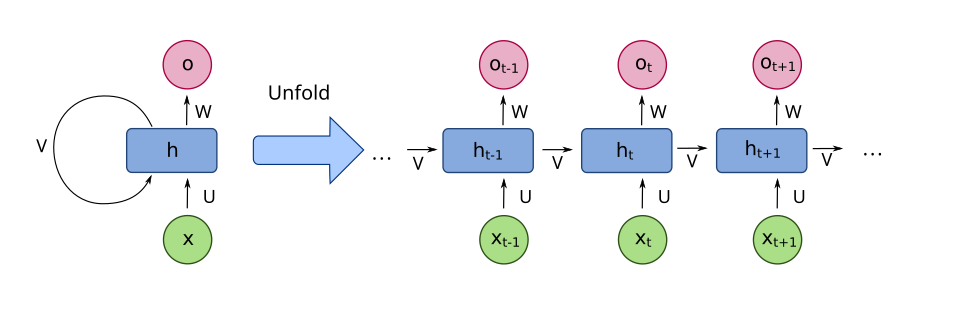
\includegraphics[width=0.82\textwidth]{figures/Recurrent_neural_network_unfold.png}
  \caption{Unfolded recurrent neural network processing a sequence through a hidden state. Source: \cite{fdeloche2017rnnunfold}.}
  \label{fig:rnn-unfolding}
\end{figure}

The basic recurrent idea is to represent time
implicitly through feedback in the hidden representation
\cite{elman1990finding}. At sequence position \(\ell\), a recurrent model can be
written as
\[
  h_\ell = \psi(x_\ell,h_{\ell-1}),
\]
where \(x_\ell\) is the current input and \(h_{\ell-1}\) summarizes the previous
part of the sequence. The hidden state is therefore a learned memory of the
past. A forward unidirectional recurrence processes the input window from its
oldest observation toward its most recent one.

A bidirectional recurrent network processes the supplied sequence in both
directions and combines the forward and backward representations
\cite{schuster1997bidirectional}. For a prediction issued at \(t_i\), both
directions can operate on the fully observed context
\(X_i=[S_{i-L+1},\ldots,S_i]\). The backward recurrence then uses observations
that are later than an internal window position, but all of them are already
available at \(t_i\). Bidirectional encoding of this past context is therefore
compatible with the no-leakage constraint. The relevant boundary is the time at
which the prediction is issued: using \(S_j\) with \(j>i\) to make that
prediction would violate the constraint. Likewise, a representation computed
using the entire window cannot be treated as available at an earlier position
inside that window if it depends on observations acquired after that position.

Plain recurrent networks can have difficulty learning long dependencies because
gradients may vanish or explode during backpropagation through time. Gated
architectures address this by controlling how information is stored and
updated. Long short-term memory networks introduced explicit memory cells and
gates \cite{hochreiter1997long}. Gated recurrent units simplify this idea while
retaining gates that regulate state updates.

\begin{figure}[htbp]
  \centering
  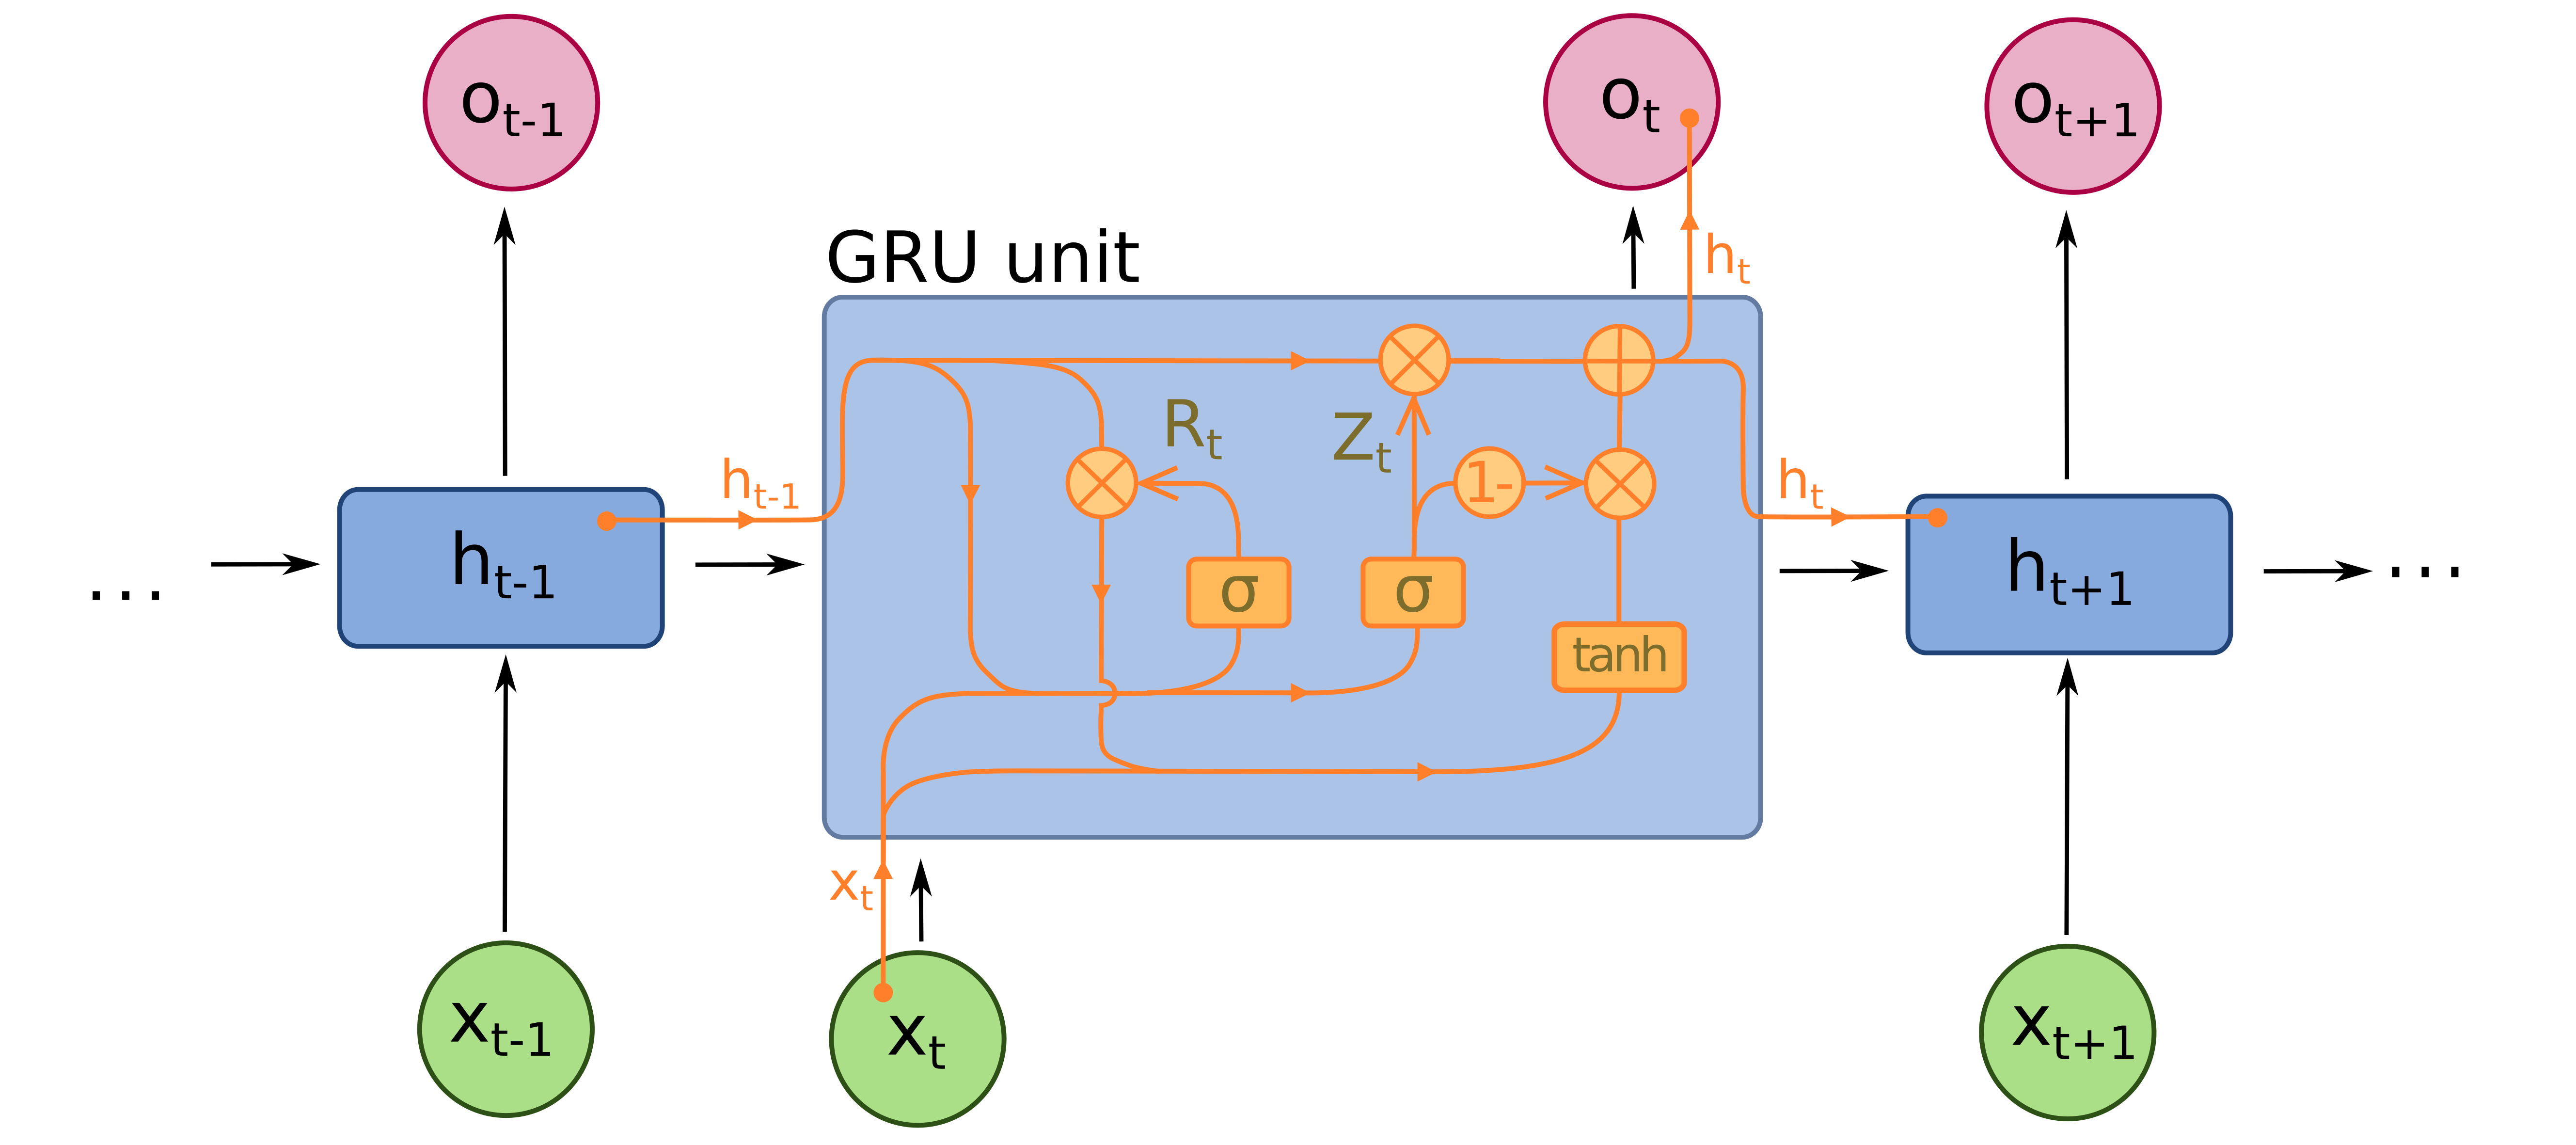
\includegraphics[width=0.82\textwidth]{figures/Gated_Recurrent_Unit.png}
  \caption{Structure of a gated recurrent unit. Source: \cite{fdeloche2017gru}.}
  \label{fig:gru-structure}
\end{figure}

GRUs were introduced in the context
of encoder-decoder sequence learning \cite{cho2014learning} and later evaluated
as general sequence modeling units \cite{chung2014empirical}.

Throughout this thesis, \(\sigma(\cdot)\) denotes the logistic sigmoid function,
\[
  \sigma(z)=\frac{1}{1+\exp(-z)},
\]
applied elementwise when its argument is a vector.

For a univariate input value \(x_t\), a GRU updates its hidden state
\(h_t\) using an update gate \(z_t\), a reset gate \(r_t\), and a
candidate state \(\widetilde{h}_t\):
\[
\begin{aligned}
  z_t &= \sigma(W_z x_t + U_z h_{t-1} + b_z), \\
  r_t &= \sigma(W_r x_t + U_r h_{t-1} + b_r), \\
  \widetilde{h}_t
  &= \tanh(W_h x_t + U_h(r_t \odot h_{t-1}) + b_h), \\
  h_t
  &= (1-z_t)\odot h_{t-1} + z_t\odot\widetilde{h}_t .
\end{aligned}
\]
The update gate controls how much of the candidate state replaces the previous
state, while the reset gate controls how much previous memory is used to form
the candidate. When \(z_t\) is small, the unit mostly preserves its previous
state; when \(z_t\) is large, it updates the memory toward the new candidate.
When \(r_t\) is small, the candidate is computed with little dependence on
older memory, allowing the unit to react to a local change. When \(r_t\) is
large, the candidate can use a longer effective history. In a fade-related
signal, these gates let the model represent whether the recent pattern resembles
a rising fade, a plateau, an oscillation, or a recovery without requiring
manually defined event states.

The hidden dimension controls the capacity of this memory. A very small hidden
state may compress different temporal patterns into similar representations,
whereas a large hidden state can overfit repeated windows from a limited number
of fade episodes. Stacking multiple GRU layers increases representational power:
lower layers can encode local signal transitions, while upper layers combine
those transitions into a coarser sequence representation. Dropout
\cite{srivastava2014dropout} and early stopping \cite{prechelt1998early}
are often used to limit overfitting, but they do not replace the need
for chronological validation because neighboring windows remain highly
correlated.

Two recurrent structures are common in multi-step forecasting. A
sequence-to-vector model encodes the whole context and maps the final hidden
state directly to an output vector:
\[
  \widehat{Y}_i = W_o a_L + b_o .
\]
This is a direct multiple-output forecast: all horizons are predicted from the
same encoded context. The advantage is that errors made for early horizons do
not have to be fed back into later horizons. The limitation is that the forecast
horizon is represented mainly through the output layer, so the model does not
explicitly simulate a future recurrent trajectory.

\begin{figure}[htbp]
  \centering
  \resizebox{0.96\textwidth}{!}{%
  \begin{tikzpicture}[
      >=Latex,
      node distance=0.9cm and 1.0cm,
      sample/.style={draw, rounded corners, align=center, minimum width=1.55cm, minimum height=0.75cm},
      block/.style={draw, rounded corners, align=center, minimum width=2.35cm, minimum height=0.95cm},
      vector/.style={draw, rounded corners, align=center, minimum width=2.75cm, minimum height=0.8cm}
    ]
    \node[sample] (x1) {\(x_1\)};
    \node[sample, right=0.25cm of x1] (x2) {\(\cdots\)};
    \node[sample, right=0.25cm of x2] (x3) {\(x_L\)};
    \node[block, right=0.95cm of x3] (encoder) {Recurrent\\encoder};
    \node[block, right=0.95cm of encoder] (state) {Final hidden\\state \(a_L\)};
    \node[block, right=0.95cm of state] (head) {Output\\mapping};
    \node[vector, right=0.95cm of head] (forecast) {\(\widehat{y}_{1:h}\)};

    \draw[->] (x1.east) -- (x2.west);
    \draw[->] (x2.east) -- (x3.west);
    \draw[->] (x3.east) -- (encoder.west);
    \draw[->] (encoder.east) -- (state.west);
    \draw[->] (state.east) -- (head.west);
    \draw[->] (head.east) -- (forecast.west);

    \node[align=center, above=0.35cm of encoder] {Input sequence};
    \node[align=center, above=0.35cm of forecast] {All horizons predicted together};
  \end{tikzpicture}%
  }
  \caption{Generic sequence-to-vector recurrent forecaster. The input sequence is encoded once, and the final hidden state is mapped directly to a multi-step output vector.}
  \label{fig:sequence-to-vector-forecasting}
\end{figure}

An encoder-decoder model instead uses one recurrent network to encode the
observed context and another to decode future values step by step, following the
broader sequence-to-sequence framework \cite{sutskever2014sequence}. The decoder
state evolves over the prediction horizon,
\[
  d_k = \psi_{\mathrm{dec}}(\xi_k,d_{k-1}),
  \qquad
  \widehat{S}_{i+k}=W_d d_k+b_d ,
\]
where \(\xi_k\) is the decoder input at future step \(k\). During training,
\(\xi_k\) may be the previous true target value, a previous prediction, or a
mixture of the two, depending on the teacher-forcing strategy. During
evaluation, future true values are unavailable, so decoded predictions must be
generated using only the encoded context and previously generated outputs. This
gives the forecast horizon an explicit temporal structure, but it can also
propagate early prediction errors.

\begin{figure}[htbp]
\centering

\begin{tikzpicture}[
    >=Latex,
    sample/.style={
        draw,
        rounded corners,
        align=center,
        minimum width=1.35cm,
        minimum height=0.7cm
    },
    block/.style={
        draw,
        rounded corners,
        align=center,
        minimum width=2.15cm,
        minimum height=0.9cm
    },
    forecastout/.style={
        draw,
        rounded corners,
        align=center,
        minimum width=1.4cm,
        minimum height=0.7cm
    }
]

% ------------------------------------------------
% Encoder
% ------------------------------------------------

\node[sample] (x1) at (-4.8, 1.3) {\(x_1\)};
\node[sample] (x2) at (-3.15, 1.3) {\(\cdots\)};
\node[sample] (x3) at (-1.5, 1.3) {\(x_L\)};

\node[block] (encoder) at (0.8, 1.3)
    {Recurrent\\encoder};

\node[block] (d0) at (3.7, 1.3)
    {Initial decoder\\state};

\node[align=center] at (-3.0, 2.15)
    {Input sequence};

% ------------------------------------------------
% Decoder
% ------------------------------------------------

\node[align=center, font=\small] at (0.2, -0.05)
    {Output sequence decoded step by step};

\node[block] (dec1) at (-3.2, -1.35)
    {Decoder\\step \(1\)};

\node[block] (dec2) at (0, -1.35)
    {Decoder\\step \(2\)};

\node[block] (dech) at (3.2, -1.35)
    {Decoder\\step \(h\)};

% ------------------------------------------------
% Outputs
% ------------------------------------------------

\node[forecastout] (y1) at (-3.2, -2.65)
    {\(\widehat{y}_1\)};

\node[forecastout] (y2) at (0, -2.65)
    {\(\widehat{y}_2\)};

\node[forecastout] (yh) at (3.2, -2.65)
    {\(\widehat{y}_h\)};

% ------------------------------------------------
% Connections
% ------------------------------------------------

\draw[->] (x1.east) -- (x2.west);
\draw[->] (x2.east) -- (x3.west);
\draw[->] (x3.east) -- (encoder.west);
\draw[->] (encoder.east) -- (d0.west);

% Initial decoder state -> first decoder step
\draw[->]
    (d0.south)
    -- ++(0,-0.45)
    -| (dec1.north);

% Autoregressive decoder evolution
\draw[->] (dec1.east) -- (dec2.west);
\draw[densely dotted] (dec2.east) -- (dech.west);

% Decoder outputs
\draw[->] (dec1.south) -- (y1.north);
\draw[->] (dec2.south) -- (y2.north);
\draw[->] (dech.south) -- (yh.north);

\end{tikzpicture}

\caption{Generic encoder-decoder recurrent forecaster.
The encoder summarizes the input sequence, while the decoder evolves over
the forecast horizon and emits one output at each step.}
\label{fig:encoder-decoder-forecasting}
\end{figure}

Compared with tree-based lag models, GRUs encode temporal order directly and
share recurrent parameters across positions in the window. This learned memory
of the available signal history makes them a natural baseline for testing
whether explicit sequence modeling improves over tabular lag features in
satellite fade nowcasting.

\subsection{Transformers and PatchTST}
\label{sec:background-patchtst}

Transformers represent sequences through attention rather than recurrence. The
core operation is scaled dot-product attention \cite{vaswani2017attention}:
\[
  \operatorname{Attention}(Q,K,V)
  =
  \operatorname{softmax}
  \left(
    \frac{QK^\top}{\sqrt{d_k}}
  \right)V .
\]
Queries, keys, and values are learned projections of input tokens. Attention
allows each token representation to combine information from other tokens in
the context.

This mechanism can now be compared with the GRU encoders introduced above.
A GRU updates its hidden state sequentially across context positions, whereas
a Transformer encoder can compute representations for all observed context
tokens in parallel within each layer \cite{vaswani2017attention}. Self-attention
also connects distant positions directly, while a recurrent encoder propagates
information through successive state updates. The GRU forecasting structures
described above summarize the context through a final recurrent state; a
Transformer encoder retains a sequence of contextualized token representations
that can be combined by the output head. The computational trade-off depends on
the context length and model dimensions, so greater parallelism alone does not
establish which model is faster for the short windows considered in this thesis.

PatchTST adapts this architecture to time-series forecasting through two design
choices: patch-based tokenization and channel-independent processing
\cite{nie2023patchtst,nixtlaPatchTSTDocs}. Instead of using one token per
timestamp, the input context is segmented into short subseries.

\begin{figure}[htbp]
  \centering
  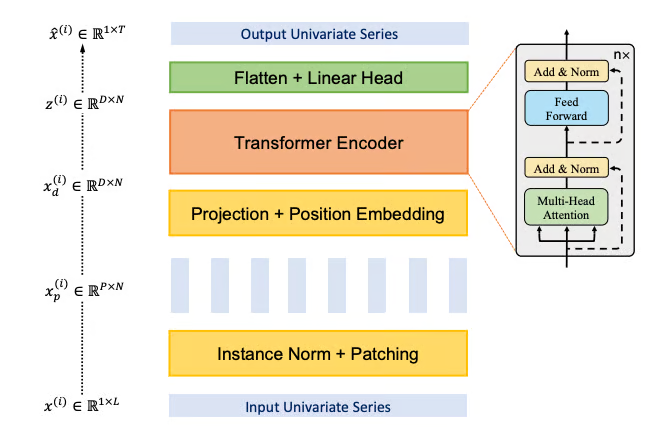
\includegraphics[width=0.78\textwidth]{figures/patchtst.png}
  \caption{PatchTST architecture for a univariate time series. The input sequence is normalized and divided into patches, embedded with positional information, processed by Transformer encoder blocks, and mapped to the output series by a linear head. Source: \cite{nie2023patchtst}.}
  \label{fig:patchtst-architecture}
\end{figure}

For a context of
length \(L\), patch length \(P\), and stride \(s\), the number of complete
patches is
\[
  N_p = 1 + \left\lfloor \frac{L-P}{s} \right\rfloor ,
\]
and the \(j\)-th patch is
\[
  p_j =
  [x_{1+(j-1)s}, \ldots, x_{1+(j-1)s+P-1}]
  \in \mathbb{R}^{P}.
\]
Each patch is projected into a \(d\)-dimensional token and combined with
positional information:
\[
  e_j = W_p p_j + b_p + r_j ,
\]
where \(W_p\) and \(b_p\) define the patch embedding and \(r_j\) encodes the
position of the patch inside the look-back window. The ordered token sequence
\([e_1,\ldots,e_{N_p}]\) is then processed by Transformer encoder blocks, whose
self-attention layers allow the representation of one patch to depend on other
patches in the context. A forecasting head maps the encoded representation to
the prediction horizon, for example through a direct multi-output projection
\[
  \widehat{Y} = W_o \operatorname{vec}(H) + b_o,
\]
where \(H\) denotes the encoded patch sequence.

Patching changes the granularity at which attention is applied. A token no
longer represents an individual sample; it represents a local temporal segment,
such as a short rise, plateau, oscillation, or recovery. This has two practical
effects. First, the embedding can preserve local shape information before the
global attention layers are applied. Second, the attention sequence length is
reduced from \(L\) to \(N_p\), lowering the cost of self-attention for the same
look-back window. The trade-off is that the patch length and stride become
important modeling choices: large or non-overlapping patches can smooth rapid
changes, while very short or highly overlapping patches reduce the computational
advantage and may behave closer to timestamp-level tokenization.

The second defining idea of PatchTST is channel independence. In a multivariate
series, each variable is treated as a separate univariate stream, with shared
embedding and Transformer weights across channels. This avoids forcing early
cross-channel mixing and improves scalability when many variables are present
\cite{nie2023patchtst}. In the signal-only setting of this thesis, there is only
one channel, so this design reduces to a purely univariate patch encoder. This
is consistent with the no-leakage and signal-only data policy: the model can
learn temporal structure in the recent signal history without receiving
additional covariates.

Practical implementations expose additional architectural and optimization
choices. The NeuralForecast implementation, for example, parameterizes the
forecast horizon and input size, the number of encoder layers and attention
heads, embedding size, patch length, stride, dropout, learnable positional
embeddings, residual attention, and reversible instance normalization
\cite{nixtlaPatchTSTDocs}. These options are not part of the task definition
itself; they control how the PatchTST family is instantiated and tuned. For
satellite fade nowcasting, the relevant motivation is that patch-level attention
can compare local fade patterns across the recent context while still producing
a direct forecast over the operational horizon.

\subsection{Foundation Time-Series Models}
\label{sec:background-chronos}

Foundation time-series models are pretrained on broad collections of time
series and then applied to new forecasting problems with little or no
task-specific training. Chronos is one such model family
\cite{ansari2024chronos}. It scales and quantizes real-valued time-series values
into discrete tokens and uses a language-model-style architecture to generate
future tokens autoregressively.

\begin{figure}[htbp]
  \centering
  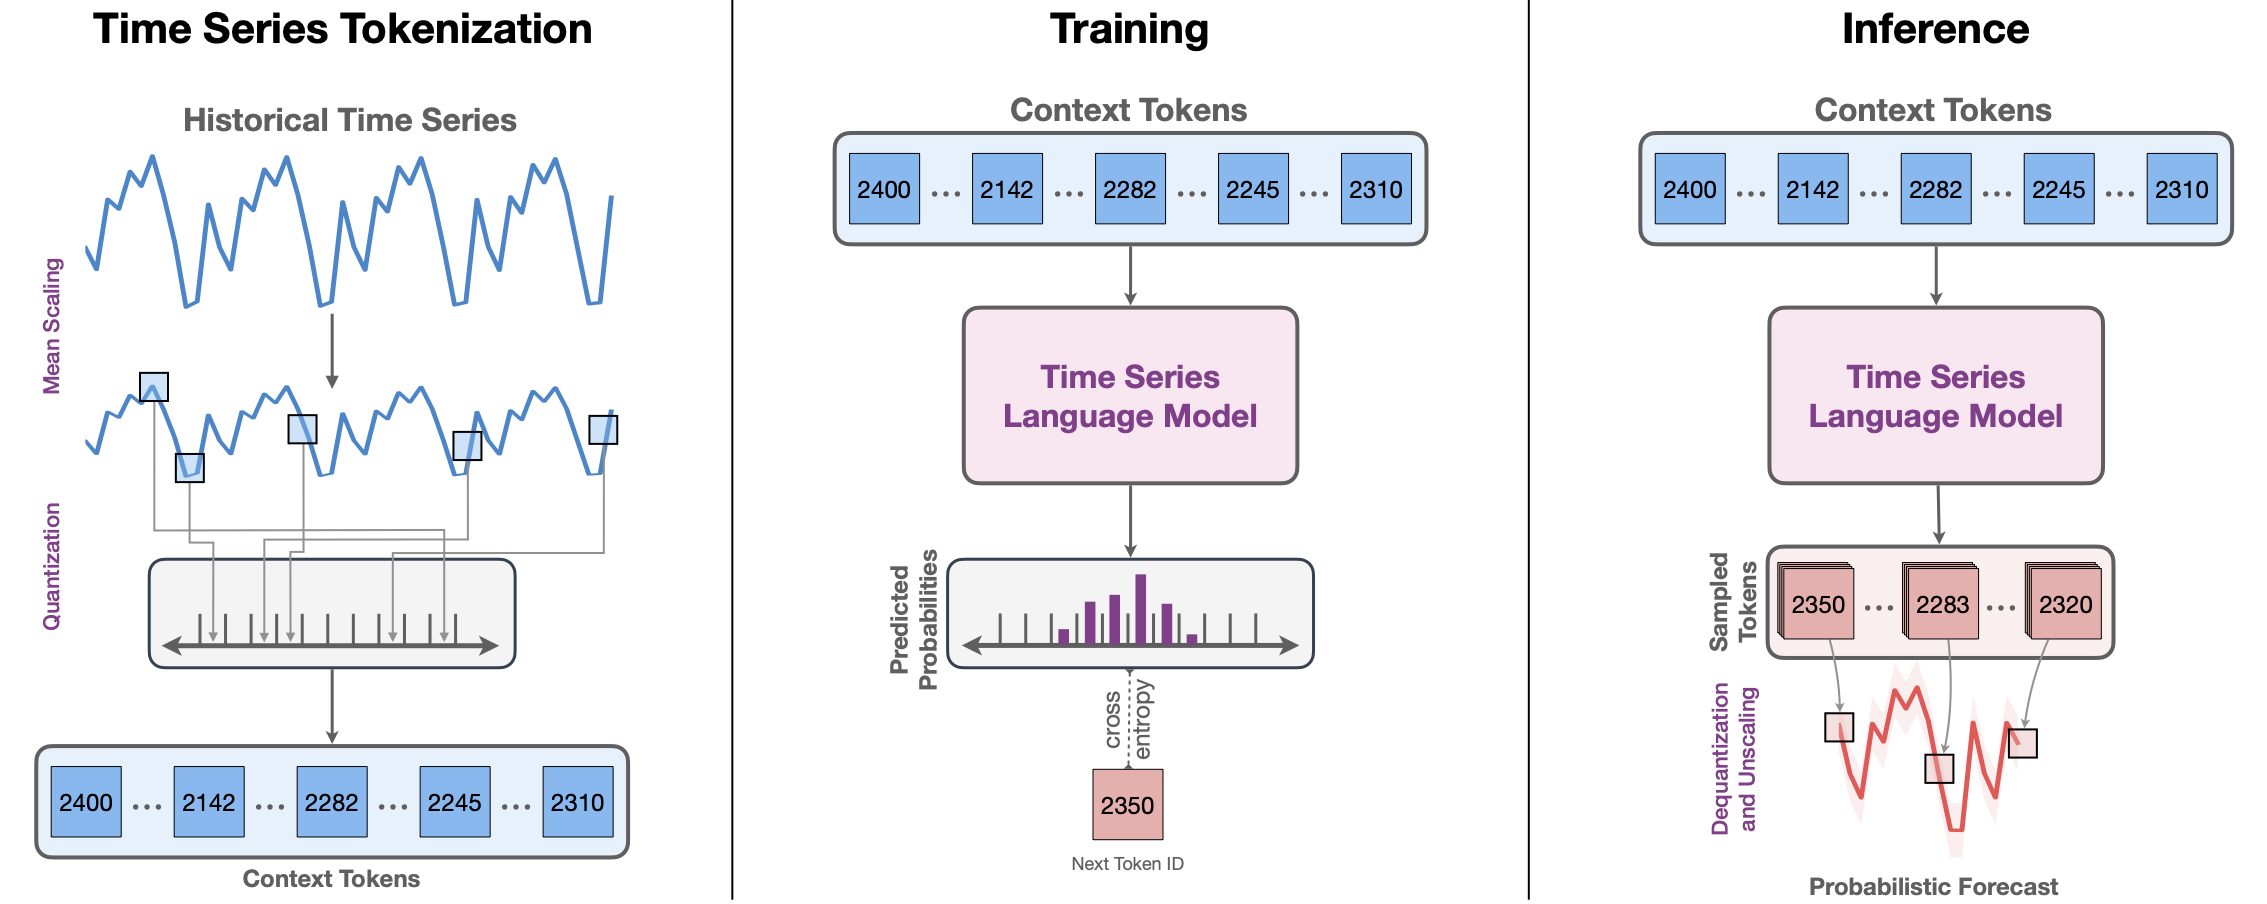
\includegraphics[width=0.95\textwidth]{figures/Chronos.png}
  \caption{High-level Chronos forecasting pipeline. The input time series is scaled and quantized into tokens, processed by a language-model architecture, and sampled autoregressively before being mapped back to numerical trajectories. Multiple sampled trajectories define a predictive distribution. Source: \cite{ansari2024chronos}.}
  \label{fig:chronos-overview}
\end{figure}

In zero-shot forecasting, a pretrained model receives only the past context from
the target series and produces a predictive distribution over future
trajectories:
\[
  p(\widehat{Y}_i \mid X_i).
\]
If multiple forecast samples are generated, a deterministic forecast can be
obtained by taking a statistic such as the median at each horizon. The main
advantage is that no project-specific parameter fitting is required. The main
limitation is domain transfer: the sampling cadence, scale, noise level, and
event structure of a satellite fade signal may differ from the data distribution
seen during pretraining.


\subsection{Temporal Convolutional Networks}
\label{sec:background-tcn}

Temporal convolutional networks use one-dimensional convolutions over ordered
sequences. A temporal convolution applies the same local filter at different
positions in the context, so the model can detect repeated patterns regardless
of where they occur inside the look-back window. This parameter sharing gives a
different inductive bias from lag-based trees, where each lag is a separate
feature, and from recurrent networks, where a hidden state is updated
sequentially.

Let \(x_t\in\mathbb{R}^{C_{\mathrm{in}}}\) be the input vector at sequence
position \(t\). A causal convolution with kernel size \(K\), dilation \(d\), and
output channel \(r\) can be written as
\[
  y_{t,r}
  =
  b_r
  +
  \sum_{c=1}^{C_{\mathrm{in}}}
  \sum_{a=0}^{K-1}
  W_{a,c,r}\,x_{t-ad,c}.
\]
The index \(t-ad\) is never greater than \(t\). The representation at position
\(t\) therefore depends only on current and past samples, which is the key
causality requirement for online nowcasting. In practice, causal convolution is
implemented with left padding or by trimming the output so that future samples
are never included in the receptive field.

The dilation factor spaces the filter taps apart. With \(d=1\), the convolution
uses adjacent samples \((x_t,x_{t-1},\ldots)\). With \(d=2\), it uses every
second sample \((x_t,x_{t-2},\ldots)\), and so on. Dilated causal convolutions
were popularized in sequence generation models such as WaveNet
\cite{oord2016wavenet}. Their advantage is that the receptive field can grow
rapidly without requiring very large kernels or very deep recurrent unrolling.

The receptive field is the part of the past that can influence an output. For a
stack of dilated convolutional layers with kernel sizes \(K_\ell\) and dilations
\(d_\ell\), assuming unit stride, the receptive field length is
\[
  R
  =
  1 + \sum_{\ell} (K_\ell-1)d_\ell .
\]
If a TCN block contains two convolutions with a common kernel size \(K\), and the
blocks use exponentially increasing dilations \(d_b=2^b\) for
\(b=0,\ldots,B-1\), the receptive field becomes
\[
  R
  =
  1 + 2(K-1)\sum_{b=0}^{B-1}2^b
  =
  1 + 2(K-1)(2^B-1).
\]
This formula makes an important modeling constraint explicit: a TCN can use
only the history covered by its receptive field. If \(R<L\), the earliest part
of a length-\(L\) context cannot affect the final output. If \(R\) is much larger
than the context, part of the nominal receptive field is filled by padding
rather than observed data.

A standard TCN is built from residual temporal blocks
\cite{bai2018tcn}. A block receives a sequence representation
\(H^{(b-1)}\in\mathbb{R}^{L\times C_b}\), applies causal dilated convolutions,
nonlinearities, normalization, and dropout, and adds the result back to the
input:
\[
  H^{(b)}
  =
  H^{(b-1)} + f_b(H^{(b-1)}).
\]
When the number of channels changes, a \(1\times 1\) convolution can project the
residual path to the correct dimension before the addition. The residual
connection helps optimization because each block learns a correction to the
previous representation instead of having to relearn the entire transformation.
Dropout and weight normalization are commonly used to stabilize training and
reduce overfitting in stacked convolutional sequence models.

\begin{figure}[htbp]
  \centering
  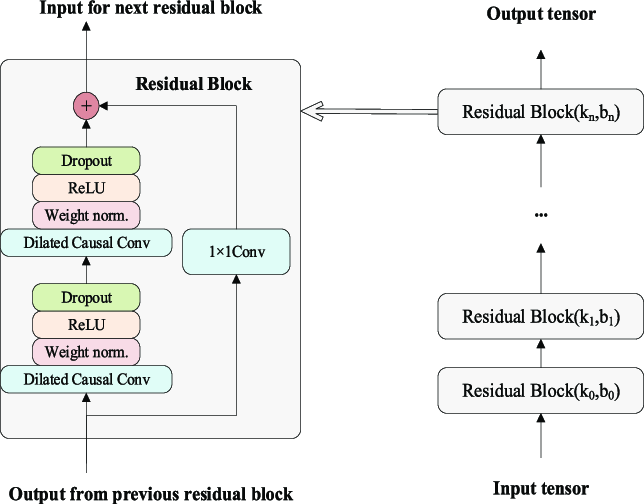
\includegraphics[width=0.72\textwidth]{figures/Architecture-of-temporal-convolutional-neural-networks-TCNs.png}
  \caption{Example architecture of a temporal convolutional network. Temporal convolutional blocks combine one-dimensional convolutions, nonlinear transformations, and residual connections to build sequence representations over a finite receptive field. Source: \cite{zhang2022attentionTcnRnn}.}
  \label{fig:tcn-architecture}
\end{figure}

For a sequence-level prediction, the final temporal representation must be
converted into a fixed-dimensional vector. Common choices include using the last
causal position, applying average or maximum pooling over time, or concatenating
several pooled summaries. The last-position representation is the most directly
causal for a decision at the end of the context, while temporal pooling can make
the model more sensitive to patterns that occurred anywhere in the look-back
window. For pointwise sequence outputs, such as a hazard at each future time bin
in a discrete-time survival model, the convolutional representation can instead
be mapped to a vector of horizon-specific logits.

TCNs occupy an intermediate position between recurrent and attention-based
models. Like GRUs, they can be made causal and are well suited to online
prediction. Unlike GRUs, they process all positions in parallel during training
and do not compress the entire past through a single recurrent state. Like
Transformers, they support parallel computation over the sequence, but their
dependency pattern is local and controlled by the receptive field rather than by
global self-attention. This makes them attractive when the relevant information
is expected to lie in local temporal shapes, slopes, threshold crossings, and
short persistence patterns. Their main limitation is that long-range dependence
must be covered deliberately through the choice of kernel size, dilation
schedule, and number of blocks; otherwise, distant samples are simply outside
the model's effective view.

In satellite fade nowcasting, this inductive bias is useful because many
operational cues are local but not instantaneous. A single sample above a
threshold may be ambiguous, whereas a short pattern of rising signal values,
oscillation near the threshold, or sustained exceedance can indicate a different
event regime. A causal TCN can learn filters for these patterns and combine
them across multiple temporal scales while preserving the no-leakage constraint.
This is why TCNs are suitable both for event classification and for
discrete-time hazard prediction, where the model must summarize recent history
before estimating the probability of future persistence or recovery.


\subsection{Shapelet-Based Time-Series Modeling}
\label{sec:background-shapelets}

A time-series shapelet is a short subsequence whose presence, absence, or
distance to a larger series is informative for prediction. Shapelets were
introduced as discriminative subsequences for interpretable time-series data
mining \cite{ye2009shapelets}. Shapelet transformations then made it possible
to use distances to selected shapelets as features for downstream classifiers
\cite{hills2014shapeletTransform}.

\begin{figure}[htbp]
  \centering
  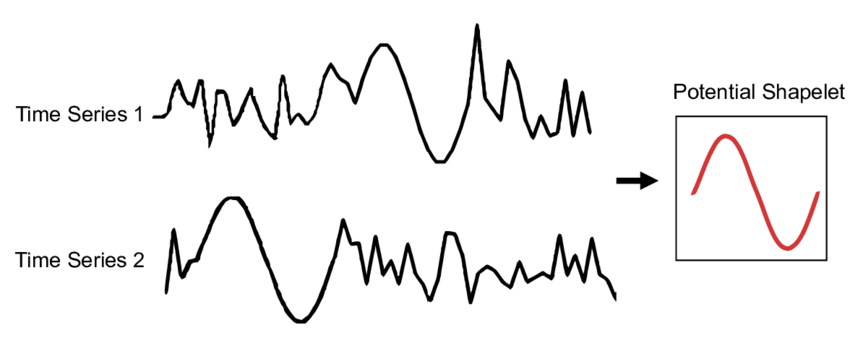
\includegraphics[width=0.85\textwidth]{figures/Time-series-shapelets.png}
  \caption{Illustration of time-series shapelets as local subsequences that are informative for distinguishing temporal patterns. Source: \cite{arul2020shapeletTransform}.}
  \label{fig:time-series-shapelets}
\end{figure}

Given a shapelet \(w\in\mathbb{R}^{\ell}\) and a context
\(x\in\mathbb{R}^{L}\), a standard squared-distance response is
\[
  d(x,w)
  =
  \min_{a=1,\ldots,L-\ell+1}
  \sum_{r=1}^{\ell}
  \left(x_{a+r-1}-w_r\right)^2 .
\]
The minimum over positions makes the feature approximately phase independent:
the pattern may appear early or late in the context and still produce a small
distance. This is useful for fade-related modeling because rapid rises,
temporary plateaus, partial recoveries, or oscillations around a threshold can
be informative even when they are not perfectly aligned across events.

The original shapelet approach searched over candidate subsequences and
selected discriminative patterns. Learnable shapelets instead treat the patterns
as differentiable model parameters optimized jointly with the prediction head
\cite{grabocka2014learning}. Multiscale learnable shapelets extend this idea by
using several shapelet lengths, allowing the model to represent both short
local transitions and longer local persistence patterns.


\subsection{Survival Analysis for Time-to-Recovery Modeling}
\label{sec:background-survival}

Survival analysis studies time-to-event outcomes in the presence of censoring.
Classical foundations include the Kaplan-Meier estimator for incomplete
observations \cite{kaplan1958nonparametric} and Cox regression models for
life-table data \cite{cox1972regression}. Let \(T\) be the true event time and
\(C\) the censoring time. The censoring time is the last time up to which the
sample can be followed before observation stops or before the event status
becomes unobservable. In this thesis, for example, a fade recovery is censored
when the acquisition segment ends before the end of the ongoing fade can be
seen. The observed time is
\[
  Y = \min(T,C),
\]
and the event indicator is
\[
  \Delta = \mathbb{1}[T \le C].
\]
If \(\Delta=0\), the event has not been observed by time \(Y\), so the valid
statement is that \(T>Y\). This is right censoring.

\begin{figure}[htbp]
  \centering
  \resizebox{\textwidth}{!}{%
  \begin{tikzpicture}[
      >=Latex,
      timeline/.style={thick, ->},
      event/.style={thick, blue!70},
      censored/.style={thick, red!70, dashed},
      marker/.style={circle, fill=black, inner sep=1.5pt},
      curve/.style={thick, blue!70},
      axis/.style={thick, ->},
      note/.style={align=center, font=\small}
    ]

    % Observed time-to-event example.
    \draw[timeline] (-6.6, 1.45) -- (-0.8, 1.45) node[right] {time};
    \draw[event] (-5.9, 1.45) -- (-2.0, 1.45);
    \node[marker] at (-5.9, 1.45) {};
    \node[marker] at (-2.0, 1.45) {};
    \node[note] at (-5.9, 2.05) {event\\starts};
    \node[note] at (-2.0, 2.05) {event\\observed};
    \node[note] at (-3.95, 0.82) {observed duration \(T=Y\), \(\Delta=1\)};

    % Right-censored example.
    \draw[timeline] (-6.6, -0.75) -- (-0.8, -0.75) node[right] {time};
    \draw[event] (-5.9, -0.75) -- (-2.65, -0.75);
    \draw[censored] (-2.65, -0.75) -- (-1.35, -0.75);
    \node[marker] at (-5.9, -0.75) {};
    \node[marker] at (-2.65, -0.75) {};
    \draw[red!70, thick] (-2.65, -1.05) -- (-2.65, -0.45);
    \node[note] at (-5.9, -1.3) {event\\starts};
    \node[note] at (-2.65, -1.55) {observation\\ends at \(C\)};
    \node[note] at (-4.05, -0.12) {right-censored: \(Y=C\), \(\Delta=0\), \(T>Y\)};

    % Survival curve.
    \draw[axis] (1.2, -1.15) -- (1.2, 2.15) node[above] {\(S(u\mid X)\)};
    \draw[axis] (1.2, -1.15) -- (6.6, -1.15) node[right] {horizon \(u\)};
    \draw[curve] plot[smooth] coordinates {
      (1.25,1.65) (2.0,1.52) (2.85,1.2) (3.6,0.75) (4.45,0.35) (5.8,0.02)
    };
    \draw[dashed] (3.75, -1.15) -- (3.75, 0.68);
    \node[note] at (3.75, -1.58) {operational\\horizon};
    \node[note] at (4.9, 1.45) {probability that the\\event lasts beyond \(u\)};
  \end{tikzpicture}
  }
  \caption{Basic survival-analysis quantities. Observed samples have a known event time, while right-censored samples are only known to survive beyond the last observable time. The survival curve maps each future horizon to the probability that the event has not yet ended.}
  \label{fig:survival-analysis-concepts}
\end{figure}

The survival function is
\[
  S(u \mid X) = P(T > u \mid X),
\]
which gives the probability that the event time exceeds horizon \(u\)
given the available input \(X\). In a satellite fade setting, the event of interest can be
interpreted as recovery from an ongoing fade rather than failure or death. This
makes survival analysis suitable for residual-duration questions, because a
survival curve can answer whether the current event is likely to last beyond an
operational horizon.

\subsubsection{Accelerated Failure Time Models and XGBoost-AFT}

Accelerated failure time (AFT) models are a parametric alternative to
proportional-hazards models. Instead of modeling the hazard ratio directly,
they model the logarithm of the event time as a location model
\cite{keiding2015survival,barnwal2022xgboostAft}:
\[
  \log T_i = \mu(X_i) + \tau \epsilon_i ,
\]
where \(X_i\) is the available input for sample \(i\), \(\mu(X_i)\) is a
location term, \(\tau>0\) is a scale parameter, and \(\epsilon_i\) follows a
chosen distribution such as normal, logistic, or extreme value. In a classical
linear AFT model, \(\mu(X_i)=\beta^\top X_i\). A positive change in
\(\mu(X_i)\) multiplies the typical event time by a factor on the original
time scale, which motivates the term ``accelerated'' failure time.

The AFT formulation is useful for censored duration targets because each sample
can be represented by lower and upper bounds on its event time. If the recovery
time is observed exactly, both bounds correspond to the observed duration,
\(L_i=U_i=T_i\). If the sample is right-censored at the end of the observable
segment, the only valid statement is \(T_i>C_i\), which can be encoded as
\(L_i=C_i\) and \(U_i=\infty\). More generally, the likelihood contribution of
an interval-censored observation is the model probability that the event time
lies inside the interval:
\[
  P(L_i < T_i \le U_i \mid X_i)
  =
  F_{\epsilon}
  \left(
    \frac{\log U_i - \mu(X_i)}{\tau}
  \right)
  -
  F_{\epsilon}
  \left(
    \frac{\log L_i - \mu(X_i)}{\tau}
  \right),
\]
with the appropriate density limit used for exact observations and with the
upper cumulative term equal to one when \(U_i=\infty\). The negative
log-likelihood derived from these terms trains the model without discarding
censored samples.

XGBoost-AFT keeps the same censored-label likelihood but replaces the linear
location term with a boosted tree ensemble:
\[
  \mu(X_i) = F(\phi_i) = \sum_{m=1}^{M} f_m(\phi_i),
\]
where \(\phi_i\) is the tabular representation of the available context
\cite{xgboostAftDocs,barnwal2022xgboostAft}. This is important for the present
thesis because the survival-persistence task uses past signal windows and
scalar summaries as input, while the target is a residual fade duration that
may be censored by the end of an acquisition segment. XGBoost-AFT can therefore
learn a nonlinear mapping from the current context to the location of the
log-duration distribution while still using both observed and right-censored
training samples.

Once \(\mu(X_i)\), the scale parameter, and the error distribution are fixed,
the model implies a full conditional survival curve:
\[
  S(u\mid X_i)
  =
  P(T_i>u\mid X_i)
  =
  1 -
  F_{\epsilon}
  \left(
    \frac{\log u - \mu(X_i)}{\tau}
  \right).
\]
Thus XGBoost-AFT does not output a binary switch by itself. It first defines a
distribution over the residual duration; an operational switch decision is then
obtained by evaluating the survival probability at a chosen horizon and applying
a configured probability threshold.

Discrete-time neural survival models partition time into ordered bins and
predict a hazard probability for each bin. If \(h_k(X)\) is the conditional
event probability in bin \(k\), then the discrete survival probability after
\(K\) bins is
\[
  S_K(X)
  =
  \prod_{k=1}^{K} \left(1-h_k(X)\right).
\]
Neural discrete-time survival models can be trained with likelihood terms for
both observed and censored samples \cite{gensheimer2019nnet}. When the hazard
model is implemented with a sequence architecture, the input representation can
still be restricted to the past context while the output retains a
time-to-event interpretation.

\section{Nowcasting Problem and Validation Principles}
\label{sec:background-nowcasting}

The model families described above provide different ways to represent temporal
information. Defining a prediction problem additionally requires specifying
when a prediction is issued, which observations are available at that time, and
which unknown outcome the prediction should describe. These choices establish
the nowcasting setting and determine what constitutes a meaningful evaluation.

\subsection{Prediction at the Current Time}

Nowcasting refers to very short-range prediction from the current and recent
state of a system. In meteorology, the World Meteorological Organization
describes nowcasting as detailed local forecasting from the present to a few
hours ahead using rapidly updated observations \cite{wmo2017nowcasting}.
The term is used here for signal-based estimates of the near-future evolution
or persistence of an ongoing satellite-link degradation, issued to support an
operational decision in the next few minutes.

At a decision time \(t_i\), the observed history supplies the information set
\(\mathcal{F}_i\), and the past context \(X_i\) is a finite representation of
that information. The target \(Y_i\) specifies the outcome to be estimated from
this information. It may concern future signal values, a remaining duration, or
an event property whose definitive label requires later observations. With model
parameters fixed for evaluation, the prediction \(z_i=f_\vartheta(X_i)\) must
be computable from information available at \(t_i\). The target can be
established retrospectively when the relevant future has been observed, or
represented as incomplete supervision when observation ends first.

The look-back duration and the prediction horizon have different roles. The
context specifies how much past information is supplied to the model; the
horizon specifies how far ahead an outcome is assessed. For a regularly sampled
forecast with interval \(\Delta\), the \(h\)-step horizon corresponds to
\(h\Delta\) units of elapsed time. A duration or survival model can instead
describe persistence over a broader range while still informing a decision at
a fixed short operational horizon. Thus, a common decision horizon does not
require every predictive task to have the same target representation.

The operational question in this thesis is whether the evolution or persistence
inferred at \(t_i\) justifies activating a backup communication link. Observing
that degradation is present does not by itself answer that question: the
unobserved continuation determines whether the interruption will be brief or
sustained. The predictive output therefore supplies evidence for a decision,
through an explicitly defined conversion rule. The satellite context is
developed in \cref{sec:background-satellite-operational}, and the alternative
targets and conversion rules are formalized in \cref{chap:task-formulations}.

\subsection{Temporal Generalization and Validation}
\label{sec:background-validation}

Evaluation must reflect the information constraints of this prediction problem.
Two distinct requirements arise: each input must respect its decision-time
boundary, and the evaluation data must test the intended form of generalization.
A past-only input is insufficient if the training and evaluation sets contain
near-duplicate windows from the same episode.

For example, a random split may place \(X_i\) in training and \(X_{i+1}\) in
testing even though they share \(L-1\) observations. Target horizons may overlap
as well. Such a split can primarily measure interpolation within already
represented episodes, whereas the operational question concerns performance on
episodes or acquisition periods that were not used to fit the model.

This does not imply that standard cross-validation is invalid for every time
series problem. Bergmeir et al. establish conditions under which it can be used
for autoregressive prediction, including uncorrelated model errors
\cite{bergmeir2018note}. Those conditions should not be assumed merely because a
time series has been stored as a table. Temporal dependence, distribution
changes, and repeated windows from the same physical episode motivate
chronological or event-grouped development splits. Holding out an entire source
dataset addresses the additional question of transfer to a different acquisition
record.

Training data are used to fit parameters. Validation data guide model and
hyperparameter selection, early stopping, and any learned decision threshold.
Test data assess the resulting fixed procedure. Transformations with fitted
parameters must follow the same separation. Changing a decision rule after
inspecting test performance makes that comparison exploratory rather than an
independent final evaluation. The concrete external-holdout construction and
experimental protocol are specified in
\cref{chap:data-reference-framework,chap:experimental-setup}.

\section{Satellite and Operational Background}
\label{sec:background-satellite-operational}

\subsection{Earth-Space Propagation and Fade Events}
\label{sec:background-earth-space-attenuation}

An Earth-space communication link is affected by deterministic link-budget terms
and by time-varying propagation impairments. The deterministic terms include
transmit power, antenna gains, free-space path loss, and receiver noise
characteristics. The time-varying terms include atmospheric gases, clouds, rain,
tropospheric scintillation, depolarization, and low-elevation effects. These
effects become increasingly important at high carrier frequencies. In Ku-, Ka-,
and V-band satellite systems, atmospheric attenuation is one of the main limits
to link availability and therefore a central design and operational concern
\cite{panagopoulos2004satellite,ippolito2017rainFadeMitigation}.

The International Telecommunication Union provides several recommendations for
Earth-space propagation engineering. Recommendation ITU-R P.618 gives methods
for propagation data and prediction in Earth-space telecommunication systems
\cite{iturP618}. Recommendation ITU-R P.837 provides precipitation statistics
used by propagation models \cite{iturP837}. Recommendation ITU-R P.1623 focuses
on fade dynamics, including fade duration and fade slope on Earth-space paths
\cite{iturP1623}, while Recommendation ITU-R P.1853 addresses synthesis of
tropospheric impairment time series \cite{iturP1853}. These documents are
important because they show that attenuation is not only a static exceedance
probability problem. Its temporal structure, including how long fades last and
how quickly they evolve, matters for systems that react dynamically.

Rain attenuation is especially relevant for short-term availability. Rain cells
can produce strong and localized signal degradation, and their movement through
the slant path causes attenuation to rise, fluctuate, and recover over time. A
classical example of dynamic rain-attenuation modeling is the stochastic model
of Maseng and Bakken \cite{maseng1981stochastic}. This thesis does not build a
physical rain model and does not use rain-rate measurements as inputs. The
propagation literature nevertheless motivates the modeling premise that recent
signal history contains information about the near-future state of the link,
while the useful information is local, noisy, and event dependent.

In the data representation used in this work, the measured column \(S_i\) is
treated as a signal or fade-level quantity. Larger values correspond to worse
link conditions. A fade region is therefore defined by an operational threshold
\[
  S_i \ge \theta .
\]
Real fade events are not perfectly smooth: the signal can cross below and above
the threshold several times during one physical degradation episode. Operational
event definitions therefore need persistence, grouping, or stable-recovery
rules rather than relying only on isolated threshold crossings.

\subsection{Fade Mitigation Techniques}

Satellite systems can respond to fading through several fade mitigation
techniques. Examples include static fade margins, uplink power control,
adaptive coding and modulation, bandwidth or data-rate adaptation, site
diversity, and switching traffic to an alternative path or backup link
\cite{panagopoulos2004satellite,ippolito2017rainFadeMitigation}. These
techniques have different physical and operational costs. Increasing transmit
power consumes power budget and may be limited by hardware or regulatory
constraints. Adaptive coding and modulation protects the link by lowering
spectral efficiency. Site diversity or backup-link switching consumes shared
network resources and can require non-negligible activation time.

Because mitigation has a cost, the operational objective is not to react to
every threshold crossing. A short isolated fade may be tolerable, while a fade
that is expected to persist for several minutes may justify early activation of
a backup resource. This turns attenuation monitoring into a short-term decision
problem: the system must use recent observations to decide whether the current
or imminent fade is persistent enough to justify action.

\subsection{Switch Decisions and Operational Metrics}
\label{sec:background-operational-evaluation}

The final operational decision considered in the thesis is binary: switch or do
not switch. Different predictive tasks may estimate different intermediate
quantities before that decision is made. A forecasting model estimates future
signal values, a duration model estimates persistence time, a classifier
estimates an event probability, and a survival model estimates a residual
duration curve. These outputs are not directly comparable until each is
converted into a binary switch sequence.

This separation between model output and switch rule is important. A model can
have a low native predictive loss but still produce poor operational behavior
if its errors occur near the threshold, if it triggers too many short switch
islands, or if it activates too late inside a fade. Conversely, a model with
moderate native error can be operationally useful if it makes reliable decisions
near the switch boundary.

For this reason, this thesis distinguishes between native predictive metrics and
operational switch metrics. Native metrics evaluate the intermediate quantity
predicted by a model. Switch metrics evaluate the binary decision sequence after
task-specific conversion and common post-processing.

For real-valued forecasting or duration regression, the main error measures are
mean absolute error and root mean squared error. Given targets \(y_i\) and
predictions \(\widehat{y}_i\), they are
\[
  \operatorname{MAE}
  =
  \frac{1}{N}
  \sum_{i=1}^{N}
  \left|\widehat{y}_i-y_i\right|,
\]
and
\[
  \operatorname{RMSE}
  =
  \sqrt{
  \frac{1}{N}
  \sum_{i=1}^{N}
  \left(\widehat{y}_i-y_i\right)^2
  } .
\]
MAE gives the average absolute error in the physical unit of the target. RMSE
penalizes large errors more strongly because the residuals are squared before
averaging. In multi-step forecasting, these quantities can also be computed by
horizon step, replacing the single target \(y_i\) with
\(y_{i,k}\), \(k=1,\ldots,h\).

For binary classification, let \(q_i\in[0,1]\) be the predicted probability and
\(y_i\in\{0,1\}\) the true class. A probability threshold converts \(q_i\) into a
class prediction. Precision, recall, and F1 are then defined from the confusion
counts
\[
\begin{aligned}
  TP &= \sum_i \mathbb{1}[\widehat{y}_i=1 \land y_i=1], &
  FP &= \sum_i \mathbb{1}[\widehat{y}_i=1 \land y_i=0], \\
  TN &= \sum_i \mathbb{1}[\widehat{y}_i=0 \land y_i=0], &
  FN &= \sum_i \mathbb{1}[\widehat{y}_i=0 \land y_i=1].
\end{aligned}
\]
The corresponding metrics are
\[
  \operatorname{Precision}=\frac{TP}{TP+FP},
  \qquad
  \operatorname{Recall}=\frac{TP}{TP+FN},
\]
and
\[
  F_1
  =
  \frac{
    2\,\operatorname{Precision}\,\operatorname{Recall}
  }{
    \operatorname{Precision}+\operatorname{Recall}
  } .
\]
The area under the receiver operating characteristic curve, AUROC, evaluates
the ranking of positive samples above negative samples across all possible
thresholds. The area under the precision-recall curve, AUPRC, evaluates the
precision-recall trade-off across thresholds and is often more informative when
the positive class is rare.

For survival models, the output is not a point estimate or a class probability
but a survival curve \(S(u\mid X)\). The negative log-likelihood measures how
much probability the model assigns to the observed time-to-event information.
For interval survival labels \([L_i,U_i]\), used for accelerated failure time
models, a generic contribution is
\[
  -\log P(L_i \le T_i \le U_i \mid X_i),
\]
with \(U_i=\infty\) for right-censored samples. In that case, the likelihood
term becomes the probability of surviving beyond the censoring lower bound.
Harrell's concordance index evaluates ranking quality: it is the fraction of
comparable sample pairs for which the model assigns shorter predicted survival
to the sample with the earlier observed event time. A value of \(0.5\) is
approximately random ranking, while a value near \(1\) indicates strong
ordering.

The Brier score evaluates the calibration and discrimination of survival
probabilities at a fixed horizon \(u\). In its simplest uncensored form, it is
\[
  \operatorname{BS}(u)
  =
  \frac{1}{N}
  \sum_{i=1}^{N}
  \left(
    \mathbb{1}[T_i>u] - \widehat{S}(u\mid X_i)
  \right)^2 .
\]
With censoring, inverse-probability-of-censoring weighting is commonly used to
avoid treating censored event status as known. The integrated Brier score
aggregates the horizon-wise Brier score over a range of horizons,
\[
  \operatorname{IBS}
  =
  \frac{1}{u_{\max}-u_{\min}}
  \int_{u_{\min}}^{u_{\max}} \operatorname{BS}(u)\,du,
\]
or the corresponding discrete average over evaluated time bins.

Operational switch metrics reuse the same confusion-count logic, but the
positive class is now a switch decision rather than a native task label. Let
\(m_i\in\{0,1\}\) denote the post-processed model switch and
\(p_i\in\{0,1\}\) the aligned Perfect Switch reference. The switch-level
confusion counts are
\[
\begin{aligned}
  TP &= \sum_i \mathbb{1}[m_i=1 \land p_i=1], &
  FP &= \sum_i \mathbb{1}[m_i=1 \land p_i=0], \\
  TN &= \sum_i \mathbb{1}[m_i=0 \land p_i=0], &
  FN &= \sum_i \mathbb{1}[m_i=0 \land p_i=1].
\end{aligned}
\]
In addition to precision, recall, and F1, switch evaluation reports
intersection over union,
\[
  \operatorname{IoU}=\frac{TP}{TP+FP+FN},
\]
balanced accuracy,
\[
  \operatorname{BalancedAccuracy}
  =
  \frac{1}{2}
  \left(
    \frac{TP}{TP+FN}
    +
    \frac{TN}{TN+FP}
  \right),
\]
false positive rate and false negative rate,
\[
  \operatorname{FPR}=\frac{FP}{FP+TN},
  \qquad
  \operatorname{FNR}=\frac{FN}{FN+TP}.
\]
Undefined divisions are handled explicitly rather than silently converted to
optimistic values.

Pointwise switch metrics are complemented by duration and event-level behavior
metrics. Active duration counts how many samples the model keeps the switch
active,
\[
  D_m=\sum_i m_i,
\]
or \(D_m\Delta t\) in seconds when the sampling time is \(\Delta t\). The
Perfect Switch duration is \(D_p=\sum_i p_i\), and the outage-mask duration is
the number of samples for which the observed signal itself is above the
threshold. The number of model switch islands is
\[
  N_m =
  \sum_i
  \mathbb{1}\left[m_i=1 \land (i=1 \lor m_{i-1}=0)\right].
\]
Detected events count Perfect Switch events that overlap at least one model
switch island. Missed events count Perfect Switch events without model overlap.
False switch events count model switch islands that do not overlap a Perfect
Switch event. When the onset of both the reference and the model switch island
is available, onset delay measures the model onset time relative to the
reference onset. Duration similarity is reported as
\[
  100\,\frac{D_p-|D_m-D_p|}{D_p}.
\]
These metrics connect statistical modeling to the practical behavior of a
fade mitigation system: they quantify not only whether the model is correct at
individual timestamps, but also whether it activates too long, misses events,
fragments one event into many switch islands, or reacts too late.
